\begin{wrapfigure}[0]{r}[-1cm]{3cm}
 \vspace{-5cm}
 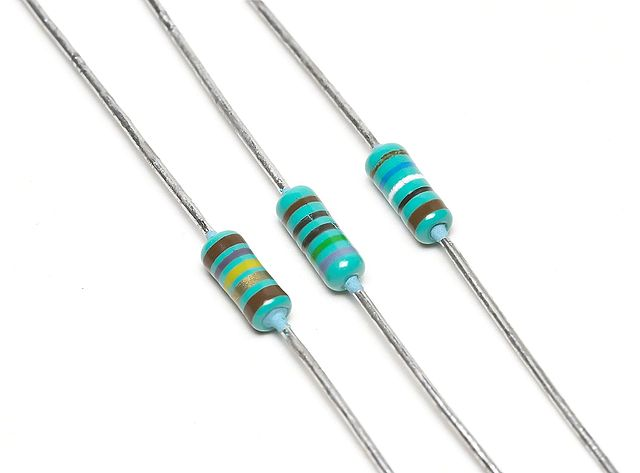
\includegraphics[scale=0.9]{Widerstand/Bilder/Resistors.jpg}
 \vspace{-5cm}
\end{wrapfigure}

\section*{Theorie- und Prüfungsfragen} 

\aufgabentext{
	\begin{enumerate}
	\item[1] \emph{\textbf{TB102}} Welchen Widerstand hat eine Kupferdrahtwicklung, wenn der verwendete Draht eine Länge von 1,8 m und einen Durchmesser von 0,2 mm hat
		\begin{enumerate}
		\itemsep1pt\parskip0pt\parsep0pt
		\item[A] 0,05 $\Omega$
		\item[B] 1 $\Omega$
		\item[C] 5,6 $\Omega$
		\item[D] 56 $\Omega$
		\loesung{Lösung: B}
		\end{enumerate}
	\end{enumerate}
}

\aufgabentext{
	\begin{enumerate}
	\item[2] \emph{\textbf{TC315}} Was verstehen Sie unter dem technischen Ausdruck Skin-Effekt?
		\begin{enumerate}
		\itemsep1pt\parskip0pt\parsep0pt
		\item[A] Als Skin-Effekt bezeichnet man die Erscheinung, dass sich mit steigender Frequenz der Elektronenstrom mehr und mehr zu den Kanten eines Kondensators hin verlagert. Dadurch erhöht sich mit steigender Frequenz die Kapazität.
		\item[B] Als Skin-Effekt bezeichnet man die Erscheinung, dass sich mit steigender Frequenz der Elektronenstrom mehr und mehr zur Oberfläche eines Leiters hin verlagert. Dadurch erhöht sich mit steigender Frequenz der Leiterwiderstand.
		\item[C] Als Skin-Effekt bezeichnet man die Erscheinung, dass sich mit steigender Frequenz die Induktivität und die Kapazität eines Leiters erhöht. Dadurch erhöht sich mit steigendem Leiterwiderstand die Resonanzfrequenz.
		\item[D] Als Skin-Effekt bezeichnet man die Erscheinung, dass sich mit steigender Frequenz der Elektronenstrom mehr und mehr zur Leitermitte hin verlagert. Dadurch erhöht sich der Leiterwiderstand bei hohem Wechselstromanteil.
		\loesung{Lösung: B}
		\end{enumerate}
	\end{enumerate}
}

\mucho{3}{TC102}
{Metallschichtwiderstände}
{haben geringe Fertigungstoleranzen und Temperaturabhängigkeit und sind besonders als Präzisionswiderstände geeignet.}
{sind induktionsarm und eignen sich besonders für den Einsatz bei sehr hohen Frequenzen.}
{sind besonders als Hochlastwiderstände bei niedrigen Frequenzen geeignet.}
{haben einen extrem stark negativen Temperaturkoeffizienten und sind besonders als NTC-Widerstände (Heißleiter) geeignet.}
{A}

\mucho{4}{TC103}
{Metalloxidwiderstände}%Frage
{haben geringe Toleranzen und Widerstandsänderungen und sind besonders als Präzisionswiderstände in der Messtechnik geeignet.}%A
{sind besonders als Hochlastwiderstände bei niedrigen Frequenzen geeignet.}%B
{sind induktionsarm und eignen sich besonders für den Einsatz bei sehr hohen Frequenzen.}%C
{haben einen extrem stark negativen Temperaturkoeffizienten und sind besonders als NTC-Widerstände (Heißleiter) geeignet.}%D
{C}%Lösung

\mucho{5}{TC104}
{Drahtwiderstände}%Frage
{Drahtwiderstände werden hauptsächlich in Form von SMD-Widerständen hergestellt.}%A
{sind induktionsarm und eignen sich besonders für den Einsatz bei sehr hohen Frequenzen.}%B
{haben einen extrem stark negativen Temperaturkoeffizienten und sind besonders als NTC-Widerstände (Heißleiter) geeignet.}%C
{sind besonders als Hochlastwiderstände bei niedrigen Frequenzen geeignet.}%D
{D}%Lösung

\mucho{6}{TB202}
{Die Leerlaufspannung  einer Gleichspannungsquelle beträgt 13,5 V. Wenn die Spannungsquelle einen Strom von 0,9 A abgibt, sinkt die Klemmenspannung auf 12,4 V. Wie groß ist der Innenwiderstand der Spannungsquelle?}%Frage
{0,82$\Omega$}%A
{1,1$\Omega$}%B
{1,22 $\Omega$}%C
{12,15 $\Omega$}%D
{C}%Lösung

\mucho{7}{TB204}
{Die Leerlaufspannung einer Gleichspannungsquelle beträgt 13,5 V. Wenn die Spannungsquelle einen Strom von 1 A abgibt, sinkt die Klemmenspannung auf 12,5 V. Wie groß ist der Wirkungsgrad der Spannungsquelle?}%Frage
{7,5 $\%$}%A
{13,5 $\%$}%B
{92,6 $\%$}%C
{100 $\%$}%D
{C}%Lösung

\mucho{8}{TB207}
{In welchem Zusammenhang müssen Innenwiderstand Ri und Lastwiderstand RL stehen, damit Leistungsanpassung vorliegt?}%Frage
{$R_L = R_i$}%A
{$R_L >> R_i$}%B
{$R_L << R_i$}%C
{$R_L = 1/R_i$}%D
{A}%Lösung

\mucho{9}{TB209}
{In welchem Zusammenhang müssen Innenwiderstand Ri und Lastwiderstand RL stehen, damit Spannungsanpassung vorliegt?}%Frage
{$R_L = R_i$}%A
{$R_L >> R_i$}%B
{$R_L << R_i$}%C
{$R_L = 1/R_i$}%D
{B}%Lösung

\mucho{10}{TB208}
{In welchem Zusammenhang müssen Innenwiderstand Ri und Lastwiderstand RL stehen, damit Stromanpassung vorliegt?}%Frage
{$R_L = R_i$}%A
{$R_L >> R_i$}%B
{$R_L << R_i$}%C
{$R_L = 1/R_i$}%D
{C}%Lösung